\chapter{Introduction}
\label{chap:intro}
\emph{Subsurface scattering} (SS) is a physical phenomenon that naturally occurs in a wide range of natural materials. Some of the materials that exhibit a strong subsurface scattering effect in everyday life are milk, human skin and marble. Subsurface scattering is that phenomenon that occurs when light is partially absorbed by an object, bounces inside ("scatters") and finally exits the surface on another point of the material (see Figure \ref{fig:ssdiagram}). The phenomenon that results is generally known as \emph{translucency}. We can see some examples of translucent objects in Figure \ref{fig:ex1}.
\section{Background}
Since the beginning of computer graphics, various attempts have been performed in order to physically model subsurface scattering. Some of these models involve Monte Carlo simulations of the light entering the medium \citep{Pharr:2000:MCE:344779.344824}, or other numerical techniques \cite{Fattal:2009:PMI:1477926.1477933,Kaplanyan:2010:CLP:1730804.1730821}. Other focus on approximating the diffusion of light within the material using an analytical approach, like \citep{Jensen:2001:PMS:383259.383319}.
 
\clearpage
\begin{figure}[!ht]
\centering
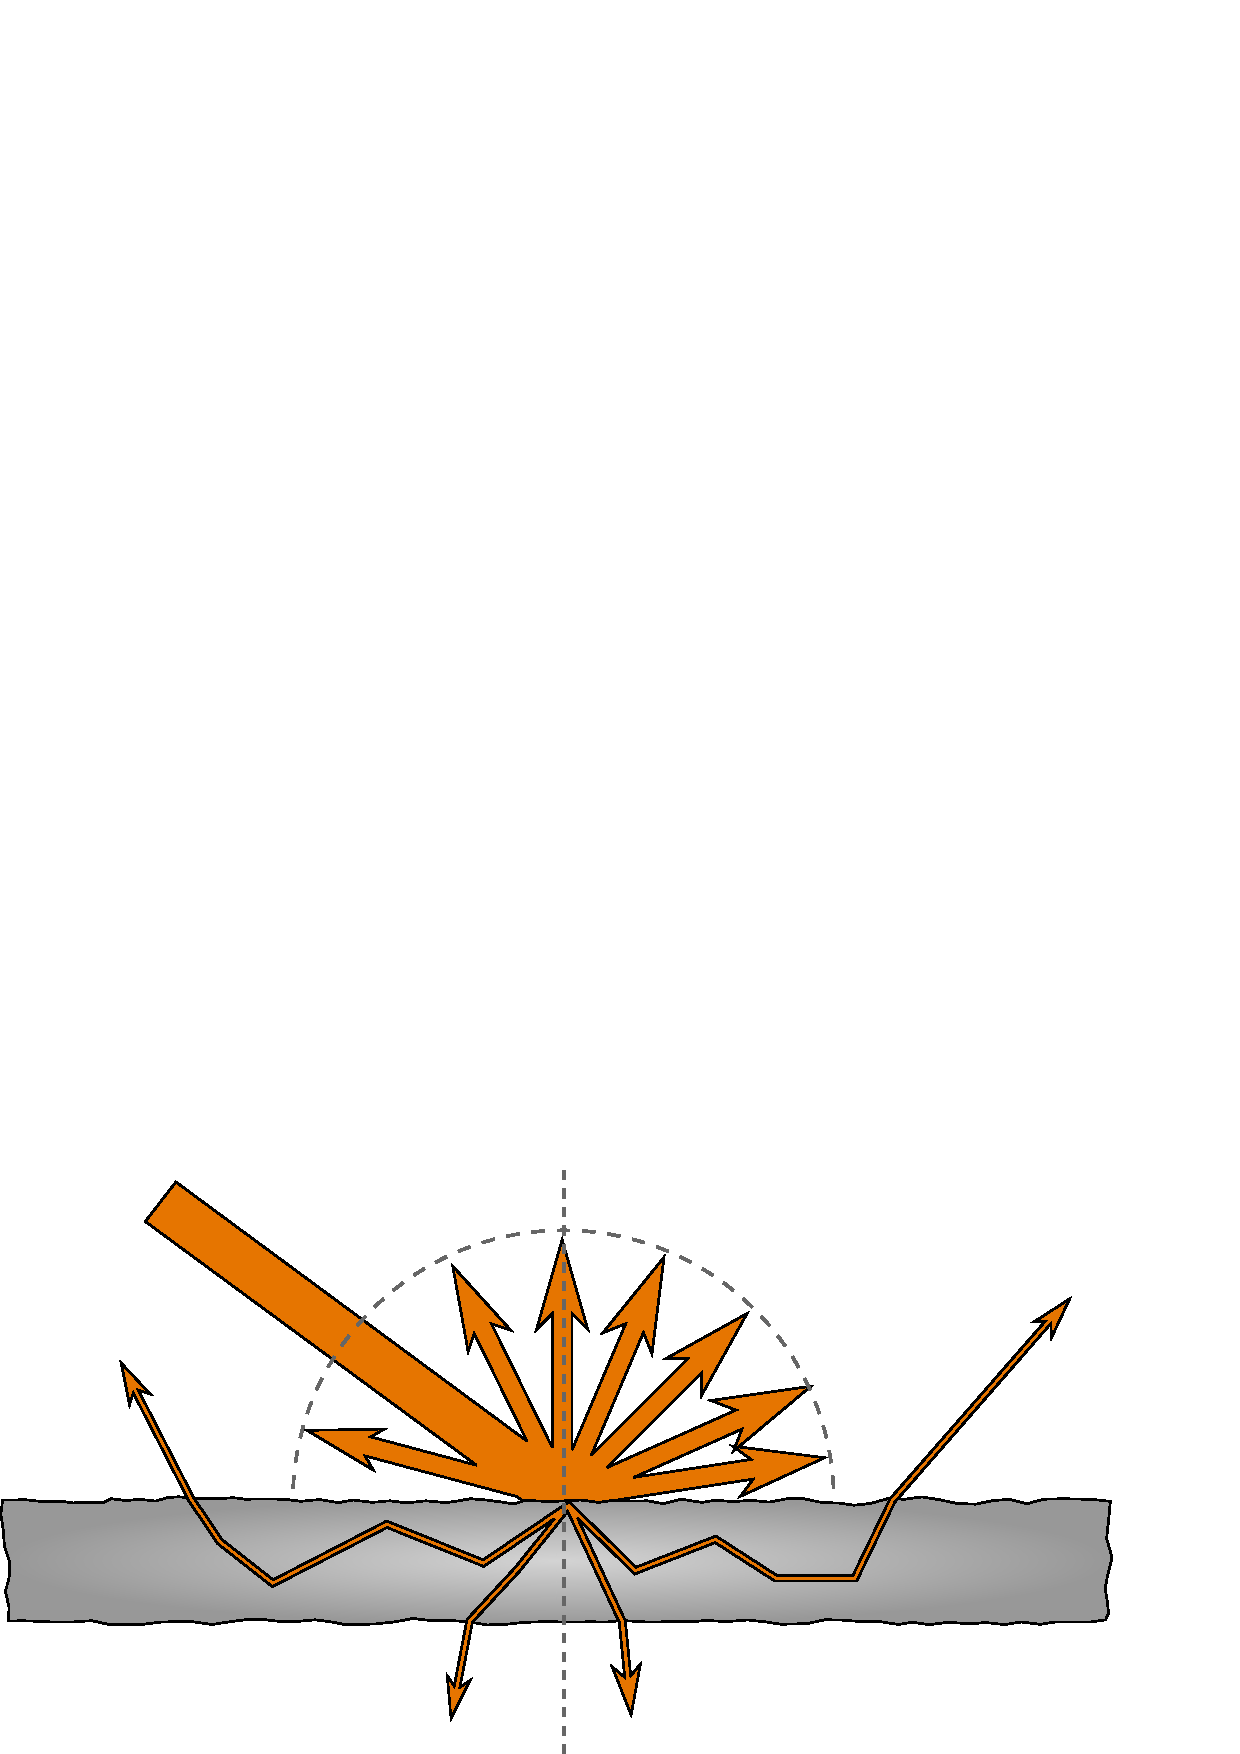
\includegraphics[width=0.8\textwidth]{images/diagram.pdf}
\caption{Diagram of subsurface scattering. Most of the incoming light gets reflected, but some of it enters the material and leaves it at a different point.}
\label{fig:ssdiagram}
\end{figure}

The first model that proposed and analytical approach was the one by \cite{Jensen:2001:PMS:383259.383319}, as an approximation of the radiative transfer equation. This approximation has then been exploited by different authors, in order to account for multi-layered materials \citep{Donner:2005:LDM:1186822.1073308}, heterogeneous materials \citep{journals/cgf/WangWHSYG10} and thin surfaces\citep{journals/cgf/WangWHSYG10}. A recent analytical approximation, proposed by \cite{IMM2013-06646}, extends the approximation in order to account for the directionality of the incoming light. All these methods are based on BSSRDF models. A BSSRDF function is a functions that describes how light is transmitted between two points in a material, and is a generally dependent on the incoming light direction, the distance between the two points and the outgoing light direction.

In recent years, with the advent of programmable graphics cards (GPU), it has become possible to exploit these algorithms and bring them to interactive frame rates, and in some cases even to real time rendering. \cite{Jensen:2002:RHR:566654.566619} were the first to propose an efficient implementation (though not real time and on a CPU) for rendering subsurface scattering using an octree. More recently, several methods have been proposed, including image-based splats, sum-of-Gaussians filtering, and grid-propagation based methods. TODO (citations). We will introduce in detail some of these method in Chapter \ref{chap:previous}, were we will review the existing literature in more detail.


\begin{figure}
\centering
\subfloat{
  \includegraphics[width= 0.9 \linewidth]{images/marble.jpg}
  \label{fig:ss1}
}
\\
\subfloat{
  \includegraphics[width= 0.9 \linewidth]{images/leaves.jpg}
  \label{fig:ss2}
} 
\\
\subfloat{
  \includegraphics[width=0.9 \linewidth]{images/candle.jpg}
  \label{fig:ss3}
} 
\caption{Some examples of translucent materials: marble, leaves and wax. The marble image and the candle are under the \href{http://creativecommons.org/licenses/by-sa/2.0/deed.en}{cc-by-sa} license, and are courtesy of Wikimedia Commons. The two images were cropped to fit the document. The leaves image was taken by Alberto Bedin and is used with permission.}
\label{fig:ex1}
\end{figure}

\section{Problem statement}

The goal of this thesis is to implement a real-time rendering technique in order to render directional subsurface scattering using the model proposed by \cite{IMM2013-06646}. The technique should ideally obtain the same results as a path traced solution of the original model, but reducing the rendering times to a few milliseconds. To do this, we propose to employ the aid of the GPU programmable pipeline \citep{Fernando:2004:GGP:983868}. 

We found that there is a current gap in the knowledge on current real-time subsurface scattering techniques regarding the approach to directional models. In fact, most of the methods rely on the assumption that the BSSRDF function depends only on the distance between the entering and exiting point \cite{Jensen:2001:PMS:383259.383319}. This allows, for example, to pre-compute the BSSRDF function and use it in the computations, greatly increasing the performance \citep{4736459}. However, in the model proposed by \cite{IMM2013-06646}, this is not possible, as the direction of the incoming light must be taken into account. In fact, the model has too many degrees of freedom to make a pre-computation feasible. 

The model proposed by \cite{IMM2013-06646} offers a more realistic evaluation of subsurface scattering effects. A real-time working implementation would improve the quality of scattering materials in real-time graphics applications, such as real-time architectural visualization and computer games. In the latter field, in recent years there has been a renewed interest in real-time SS techniques, especially to model faithfully the skin of human faces. 

\section{Requirement analysis}

In this section, we will introduce some constraints and assumptions on our method. Some of these assumptions and constraints are well known to the graphics community, and they are generally introduced to allow better performance, quality and flexibility. Being a real-time rendering method implies that performance plays a big part in the decisions made in the process, but since the method uses a physically based approximation the final quality of the result is also important. In the process the aspect of flexibility has been taken into account, i.e. the capacity of the method to set the tradeoff between quality and performance. We will now list the assumptions we made in all the three described domains, quality, performance and flexibility. 

\subsection{Quality constraints}
 \label{sec:quality}
\begin{enumerate}
	\item Being close as much as possible to a path traced solution. By \emph{close} we mean that the root mean square of the comparison between our method and a path traced result under the same lighting conditions should not be over a certain threshold. 
	\item Being consistent with the directional dipole model for a wide range of material properties. In particular, the method should perform well in the domain of quality where the directional dipole model excels (highly scattering materials).
	\item Being potentially able to render an object under an arbitrary number of lights with different properties (point, directional, environment, etc.).
\end{enumerate}

\subsection{Flexibility requirements}	
\begin{enumerate}
	\item Work with the less amount as possible of provided model data, i.e. only the position data and eventually the normals should be provided in order for the method to run. In particular, no unwrap of the mesh (UV mapping) should be necessary. In case normal data are missing,  being able to generate them using a standard method to give a smooth appearance.
	\item Be possible to be integrated in a game engine environment, using data from other computations (e.g. from other lighting computations) and being adaptable to different lighting paths (forward and deferred shading).
  \item The quality versus performance tradeoff should be set by a potential artist or developer, with the fewest number of parameters as possible.
\end{enumerate}

\subsection{Performance requirements}

\begin{enumerate}
	\item Being real-time on a high-end modern GPU, i.e. one frame should take less that 100 ms (10 FPS) to render. The ideal result would be to reach a rendering time of less than 16 ms (60 FPS).
	\item Being as less dependent as possible from the geometrical complexity of the model.
	\item Being as less dependent as possible from the screen resolution.
	\item If the desired quality is not reachable within one frame, converge towards a result in a reasonable amount of time. Techniques should be used to approximate the required quality for the intermediate result. 
	\item Maintain a reasonable performance under changing light conditions, deformations and change of parameters, with little or none performance penalties.
	\item Employ the advantages of the directional dipole model to improve performance.
	\item Support a certain number of directional and point lights (up to 3 to 5 pixel lights, as in commercial engines\citep{unitymanual}).
	\item Require little or no pre-processing in order to be able to perform. In particular, pre-processing, if any, should be general and performed only at the beginning of the life cycle of the program. 
\end{enumerate}

\section{Thesis Outline}

In this chapter, we gave an introduction to the problem and stated the assumption that will guide us to the choices that we will make through our thesis. In chapter \ref{chap:previous}, Related Work, we will describe in more detail some of the different approaches to subsurface scattering in literature. In Chapter \ref{chap:theory}, we will give a theoretical introduction to Subsurface scattering and light transport theory, with a special focus on BSSRDF functions. In chapter \ref{chap:method}, we will describe our method on approaching the problem on a theoretical basis. In Chapter \ref{chap:implementation} we will describe the actual implementation of the method, and the problems and limitations met during the process. In Chapter \ref{chap:results}, we will describe the tests we made and show the results, both in the domain of performance and quality, comparing them with the requirement analysis we made in the previous section. Finally, we will describe some possible extensions to the method in chapter \ref{chap:futurework}.  

